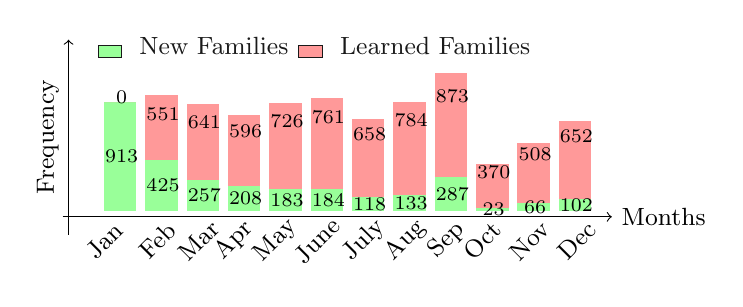
\begin{tikzpicture}[scale=1.5]

    \tikzstyle{every node}=[font=\small]
    % Scaling factor for the heights
    \def\scalefactor{0.001}
    
    % Define data for New and Learned Families
    \def\NewFamilies{{913, 425, 257, 208, 183, 184, 118, 133, 287, 23, 66, 102}}
    \def\LearnedFamilies{{0, 551, 641, 596, 726, 761, 658, 784, 873, 370, 508, 652}}

    % Define months
    \def\Months{{"Jan","Feb","Mar","Apr","May","Jun","Jul","Aug","Sep","Oct","Nov","Dec"}}
    
    % Loop through each month
    \foreach \x [count=\xi] in {0,...,11}{
        % Accessing the \x-th element of each list
        \pgfmathsetmacro\NewFamily{\NewFamilies[\x]}
        \pgfmathsetmacro\LearnedFamily{\LearnedFamilies[\x]}
        
        % Calculate bottom and top of the Learned Families bar
        \pgfmathsetmacro\NewHeight{\NewFamily*\scalefactor}
        \pgfmathsetmacro\LearnedHeight{(\NewFamily + \LearnedFamily)*\scalefactor}
        
        % Position for each month's data
        \pgfmathsetmacro\position{\xi*0.35}
        
        % Draw New Families (bottom bar)
        \fill[green!40] (\position,0) rectangle (\position+0.275,\NewHeight);
        % Draw Learned Families (stacked on top of New Families)
        \fill[red!40] (\position,\NewHeight) rectangle (\position+0.275,\LearnedHeight);
        
        % Add value labels for New and Learned Families
        \node at (\position+0.15,\NewHeight/2) {\scriptsize\NewFamily};
        % Display LearnedFamily value only if it's greater than 0
        \ifnum\LearnedFamily = 0
            \node at (\position+0.15,\LearnedHeight*1.05) {\scriptsize\LearnedFamily};
        \fi
         \ifnum\LearnedFamily > 0
            \node at (\position+0.15,\LearnedHeight/1.2) {\scriptsize\LearnedFamily};
        \fi
    }
     % Add month label below the x-axis
    %\node[rotate=45] at (\position+0.15,-0.2) {\tiny\Months[\x]};


    \node[rotate=45] at (0.35,-0.25) {Jan};
    \node[rotate=45] at (0.8,-0.25) {Feb};
    \node[rotate=45] at (1.15,-0.25) {Mar};
    \node[rotate=45] at (1.45,-0.25) {Apr};
    \node[rotate=45] at (1.80,-0.25) {May};
    \node[rotate=45] at (2.15,-0.25) {June};
    \node[rotate=45] at (2.55,-0.25) {July};
    \node[rotate=45] at (2.90,-0.25) {Aug};
    \node[rotate=45] at (3.25,-0.25) {Sep};
    \node[rotate=45] at (3.55,-0.25) {Oct};
    \node[rotate=45] at (3.95,-0.25) {Nov};
    \node[rotate=45] at (4.35,-0.25) {Dec};


    % Draw the axes
    \draw[->] (0.0,-0.05) -- (4.65,-0.05) node[right] {Months};
    \draw[->] (0.05,-0.2) -- (0.05,1.45) node[rotate=90, midway, above] {Frequency};
    

    % Add legends (moved to top right)
    \draw [black!90, fill=green!40] (.3,1.3) rectangle (0.5,1.4) node[right, xshift=0.1cm] {\small New Families};
    \draw [black!90, fill=red!40] (2.0,1.3) rectangle (2.20,1.4) node[right, xshift=0.1cm] {\small Learned Families};
    
\end{tikzpicture}

